% \documentclass[table]{beamer}
\documentclass[table,handout]{beamer}
\setbeameroption{show notes}
% \setbeameroption{hide notes}
% \setbeameroption{show only notes}
\usepackage{varwidth}

\newif\ifhide
\newif\ifpost
\newif\ifhideclicker

% \hidetrue
% \hideclickertrue
% \posttrue

\newcommand{\whiteout}[1]{\textcolor{white}{#1}}
% \newcommand{\whiteoutbox}[1]{\fcolorbox{white}{white}{\parbox{\dimexpr \linewidth-2\fboxsep-2\fboxrule}{\whiteout{#1}}}}
% \newcommand{\notebox}[1]{\fcolorbox{blue}{white}{\parbox{\dimexpr \linewidth-2\fboxsep-2\fboxrule}{#1}}}
\newcommand{\whiteoutbox}[1]{\fcolorbox{white}{white}{\parbox{\linewidth}{\whiteout{#1}}}}
\newcommand{\notebox}[1]{\fcolorbox{blue}{white}{\parbox{\linewidth}{#1}}}
\newcommand{\blankbox}[1]{\phantom{\varwidth{\linewidth}\whiteoutbox{#1}\endvarwidth}}
\newcommand{\blank}[1]{\phantom{\varwidth{\linewidth}#1\endvarwidth}}

\ifhide%
    \newcommand{\hmask}[1]{\blank{#1}}%
\else%
    \newcommand{\hmask}[1]{#1}%
\fi

\ifhide%
    \newcommand{\wout}[1]{\whiteout{#1}}%
\else%
    \newcommand{\wout}[1]{#1}%
\fi

\ifhide%
    \newcommand{\hignore}[1]{}%
\else%
    \newcommand{\hignore}[1]{#1}%
\fi

\ifpost%
    \newcommand{\nopost}[1]{}%
\else%
    \newcommand{\nopost}[1]{#1}%
\fi

\ifhideclicker%
    \newcommand{\clickerslide}[1]{\stepcounter{clickerQuestionCounter}%
        \begin{frame}[t]
            \textcolor{blue}{Q \arabic{clickerQuestionCounter}:}
        \end{frame}}
\else%
    \newcommand{\clickerslide}[1]{#1}%
\fi

\ifhide%
    \newcommand{\hidebox}[1]{\blank{#1}}%
\else%
    \newcommand{\hidebox}[1]{\notebox{#1}}%
\fi

\ifhide%
    \newcommand{\wbox}[1]{\whiteoutbox{#1}}%
\else%
    \newcommand{\wbox}[1]{\notebox{#1}}%
\fi

\ifhide%
    \newcommand{\nbox}[1]{\blankbox{#1}}%
\else%
    \newcommand{\nbox}[1]{\notebox{#1}}%
\fi

\ifhideclicker%
    \newcommand{\clickeranswer}[1]{#1}%
\else%
    \ifhide%
        \newcommand{\clickeranswer}[1]{#1}%
    \else%
        \newcommand{\clickeranswer}[1]{\textbf{\textcolor{blue}{#1}}}%
    \fi
\fi

\usepackage{beamerthemesplit}
% \usetheme{boxes}
\usetheme{Malmoe}
\usecolortheme{seahorse}
% \usecolortheme{seagull}
\usepackage{ifthen}
\usepackage{xspace}
\usepackage{multirow}
\usepackage{multicol}
\usepackage{booktabs}
\usepackage{xcolor}
\usepackage{wasysym}
\usepackage{comment}
\usepackage{hyperref}
\hypersetup{pdfborder={0 0 0}, colorlinks=true, urlcolor=blue, linkcolor=blue, citecolor=blue}
\usepackage{changepage}
\usepackage[compatibility=false]{caption}
\captionsetup[figure]{font=scriptsize, labelformat=empty, textformat=simple, justification=centering, skip=2pt}
\usepackage{tikz}
\usetikzlibrary{trees,calc,backgrounds}

\usepackage[bibstyle=joaks-slides,maxcitenames=3,mincitenames=1,backend=biber]{biblatex}

\newrobustcmd*{\shortfullcite}{\AtNextCite{\renewbibmacro{title}{}\renewbibmacro{in:}{}\renewbibmacro{number}{}}\fullcite}

\newrobustcmd*{\footlessfullcite}{\AtNextCite{\renewbibmacro{title}{}\renewbibmacro{in:}{}}\footfullcite}

% Make all footnotes smaller
% \renewcommand{\footnotesize}{\scriptsize}

\definecolor{myGray}{gray}{0.9}
\colorlet{rowred}{red!30!white}

\setbeamertemplate{blocks}[rounded][shadow=true]

\setbeamercolor{defaultcolor}{bg=structure!30!normal text.bg,fg=black}
\setbeamercolor{block body}{bg=structure!30!normal text.bg,fg=black}
\setbeamercolor{block title}{bg=structure!50!normal text.bg,fg=black}

\newenvironment<>{varblock}[2][\textwidth]{%
  \setlength{\textwidth}{#1}
  \begin{actionenv}#3%
    \def\insertblocktitle{#2}%
    \par%
    \usebeamertemplate{block begin}}
  {\par%
    \usebeamertemplate{block end}%
  \end{actionenv}}

\newenvironment{displaybox}[1][\textwidth]
{
    \centerline\bgroup\hfill
    \begin{beamerboxesrounded}[lower=defaultcolor,shadow=true,width=#1]{}
}
{
    \end{beamerboxesrounded}\hfill\egroup
}

\newenvironment{onlinebox}[1][4cm]
{
    \newbox\mybox
    \newdimen\myboxht
    \setbox\mybox\hbox\bgroup%
        \begin{beamerboxesrounded}[lower=defaultcolor,shadow=true,width=#1]{}
    \centering
}
{
    \end{beamerboxesrounded}\egroup
    \myboxht\ht\mybox
    \raisebox{-0.25\myboxht}{\usebox\mybox}\hspace{2pt}
}

\newenvironment{mydescription}{
    \begin{description}
        \setlength{\leftskip}{-1.5cm}}
    {\end{description}}

\newenvironment{myitemize}{
    \begin{itemize}
        \setlength{\leftskip}{-.3cm}}
    {\end{itemize}}

% footnote without a marker
\newcommand\barefootnote[1]{%
  \begingroup
  \renewcommand\thefootnote{}\footnote{#1}%
  \addtocounter{footnote}{-1}%
  \endgroup
}

% define formatting for footer
\newcommand{\myfootline}{%
    {\it
    \insertshorttitle
    \hspace*{\fill} 
    \insertshortauthor, \insertshortinstitute
    % \ifx\insertsubtitle\@empty\else, \insertshortsubtitle\fi
    \hspace*{\fill}
    \insertframenumber/\inserttotalframenumber}}

% set up footer
\setbeamertemplate{footline}{%
    \usebeamerfont{structure}
    \begin{beamercolorbox}[wd=\paperwidth,ht=2.25ex,dp=1ex]{frametitle}%
        % \Tiny\hspace*{4mm}\myfootline\hspace{4mm}
        \tiny\hspace*{4mm}\myfootline\hspace{4mm}
    \end{beamercolorbox}}

% remove navigation bar
\beamertemplatenavigationsymbolsempty

\makeatletter
    \newenvironment{noheadline}{
        \setbeamertemplate{headline}[default]
        \def\beamer@entrycode{\vspace*{-\headheight}}
    }{}
\makeatother

\newcounter{clickerQuestionCounter}
\ifhideclicker%
\newenvironment{clickerquestion}
{ \stepcounter{clickerQuestionCounter}
  \begin{enumerate}[Q \arabic{clickerQuestionCounter}:]\color{white} }
{ \end{enumerate} }
\else%
\newenvironment{clickerquestion}
{ \stepcounter{clickerQuestionCounter}
  \begin{enumerate}[Q \arabic{clickerQuestionCounter}:] }
{ \end{enumerate} }
\fi

\ifhideclicker%
\newenvironment{clickeroptions}
{ \begin{enumerate}[\begingroup\color{white} 1)\endgroup]\color{white} }
{ \end{enumerate} }
\else%
\newenvironment{clickeroptions}
{ \begin{enumerate}[\begingroup\color{red} 1)\endgroup] }
{ \end{enumerate} }
\fi


\tikzstyle{centered} = [align=center, text centered, font=\sffamily\bfseries]
\tikzstyle{skip} = [centered, inner sep=0pt, fill]
\tikzstyle{empty} = [centered, inner sep=0pt]
\tikzstyle{inode} = [centered, circle, minimum width=4pt, fill=black, inner sep=0pt]
\tikzstyle{tnode} = [centered, circle, inner sep=1pt]
\tikzset{
  % edge styles
  level distance=10mm,
  mate/.style={edge from parent/.style={draw,distance=3pt}},
  mleft/.style={grow=left, level distance=10mm, edge from parent path={(\tikzparentnode.west)--(\tikzchildnode.east)}},
  mright/.style={grow=right, level distance=10mm, edge from parent path={(\tikzparentnode.east)--(\tikzchildnode.west)}},
  % node styles
  male/.style={rectangle,minimum size=4mm,fill=gray!80},
  female/.style={circle,minimum size=4mm,fill=gray!80},
  amale/.style={male,fill=red},
  afemale/.style={female,fill=red},
}

\newcommand{\highlight}[1]{\textcolor{violet}{\textit{\textbf{#1}}}}
\newcommand{\super}[1]{\ensuremath{^{\textrm{\sffamily #1}}}}
\newcommand{\sub}[1]{\ensuremath{_{\textrm{\sffamily #1}}}}
\newcommand{\dC}{\ensuremath{^\circ{\textrm{C}}}}
\newcommand{\tb}{\hspace{2em}}
\providecommand{\e}[1]{\ensuremath{\times 10^{#1}}}
\newcommand{\myHangIndent}{\hangindent=5mm}

\newcommand{\spp}[1]{\textit{#1}}

\newcommand\mybullet{\leavevmode%
\usebeamertemplate{itemize item}\hspace{.5em}}

\makeatletter
\newcommand*{\rom}[1]{\expandafter\@slowromancap\romannumeral #1@}
\makeatother

\newcommand{\blankslide}{{\setbeamercolor{background canvas}{bg=black}
\setbeamercolor{whitetext}{fg=white}
\begin{frame}<handout:0>[plain]
\end{frame}}}

\newcommand{\whiteslide}{
\begin{frame}<handout:0>[plain]
\end{frame}}

\newcommand{\f}[1]{\ensuremath{F_{#1}}}
\newcommand{\x}[1]{X\ensuremath{^{#1}}}
\newcommand{\y}[1]{Y\ensuremath{^{#1}}}

% Population growth macros
\newcommand{\popsize}[1]{\ensuremath{N_{#1}}}
\newcommand{\popgrowthratediscrete}[1]{\ensuremath{\lambda_{#1}}}
\newcommand{\popgrowthrate}[1]{\ensuremath{r_{#1}}}
\newcommand{\ptime}{\ensuremath{t}\xspace}

\tikzset{hide on/.code={\only<#1>{\color{white}}}}
\tikzset{
    invisible/.style={opacity=0},
    visible on/.style={alt={#1{}{invisible}}},
    alt/.code args={<#1>#2#3}{%
        \alt<#1>{\pgfkeysalso{#2}}{\pgfkeysalso{#3}}
        % \pgfkeysalso doesn't change the path
    },
}

\bibliography{../bib/references}
\author[J.\ Oaks]{
    %Jamie R.\ Oaks\inst{1}
    Jamie R.\ Oaks
}
\institute[BIOL 180]{
    \inst{}%
        BIOL 180: Introductory Biology
}



\title[Speciation]{Speciation}
% \date{\today}
\date{April 30, 2015}

\begin{document}

\begin{noheadline}
\maketitle
\end{noheadline}

\nopost{
\begin{noheadline}
\begin{frame}[c]
    \vspace{-6mm}
    \begin{center} 
        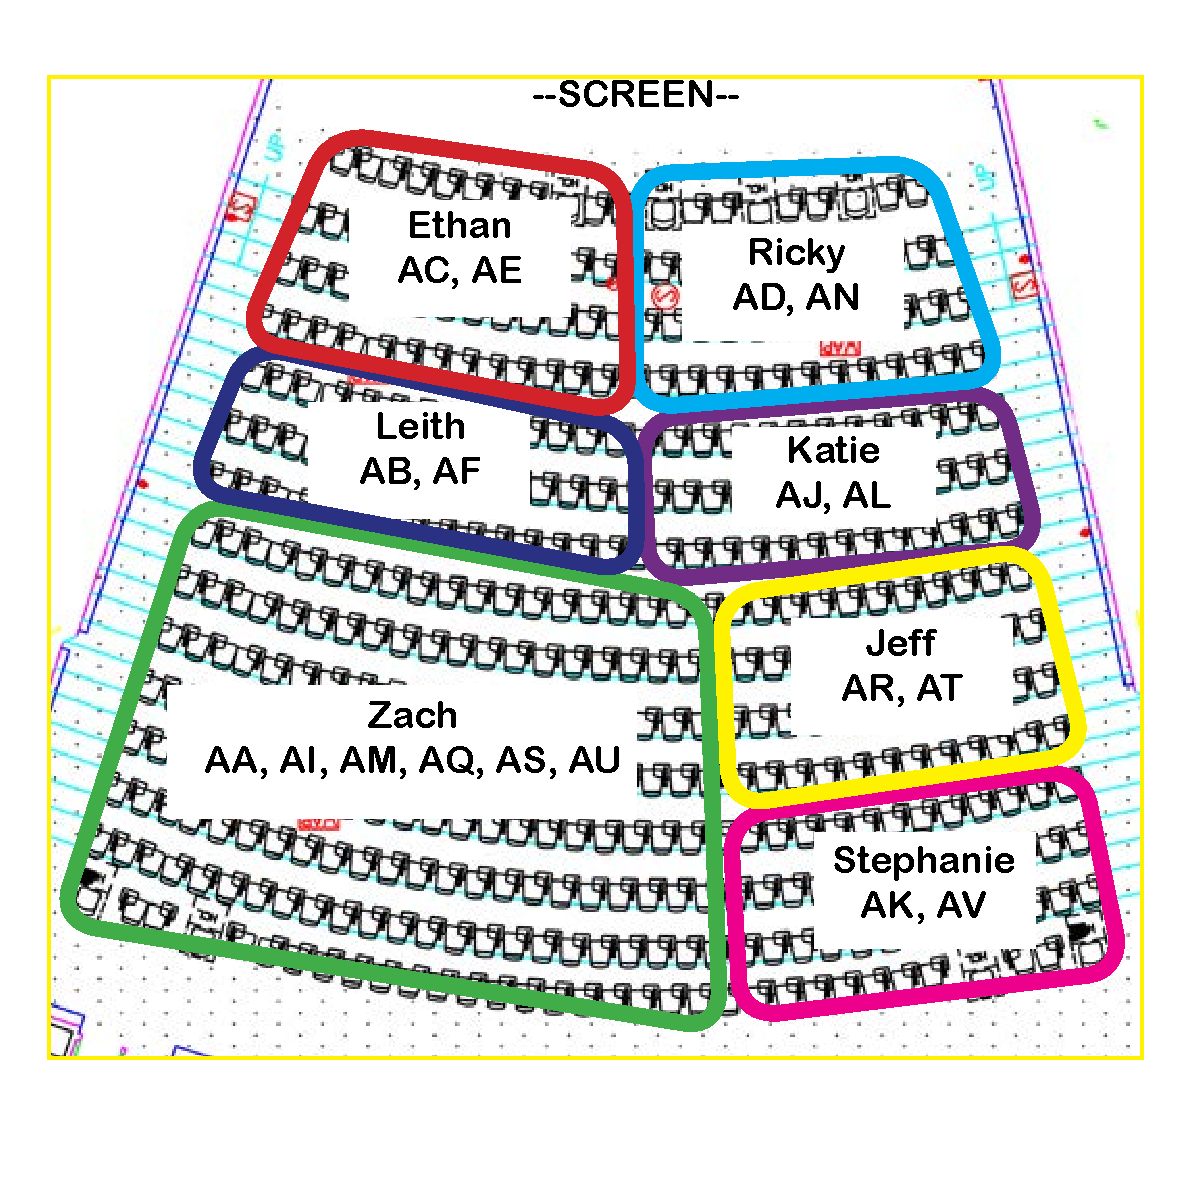
\includegraphics[height=1.2\textheight]{../images/seating-chart.pdf}
    \end{center}
\end{frame}
\end{noheadline}
}

\clickerslide{
\begin{frame}
    \begin{clickerquestion}
        \item Consider the wings of bats and birds; which of the following is
            correct?
        \begin{clickeroptions}
            \item Wings are homologous; limbs are homoplastic.
            \item Both have highly modified hand and finger bones; these
                modifications are homologous.
            \item \clickeranswer{Many genes for limb formation are homologous,
                    but the different alleles/genes that give rise to wings in
                    each are homoplastic.}
            \item None of the above.
        \end{clickeroptions}
    \end{clickerquestion}
\end{frame}
}

\clickerpost{
{
\usebackgroundtemplate{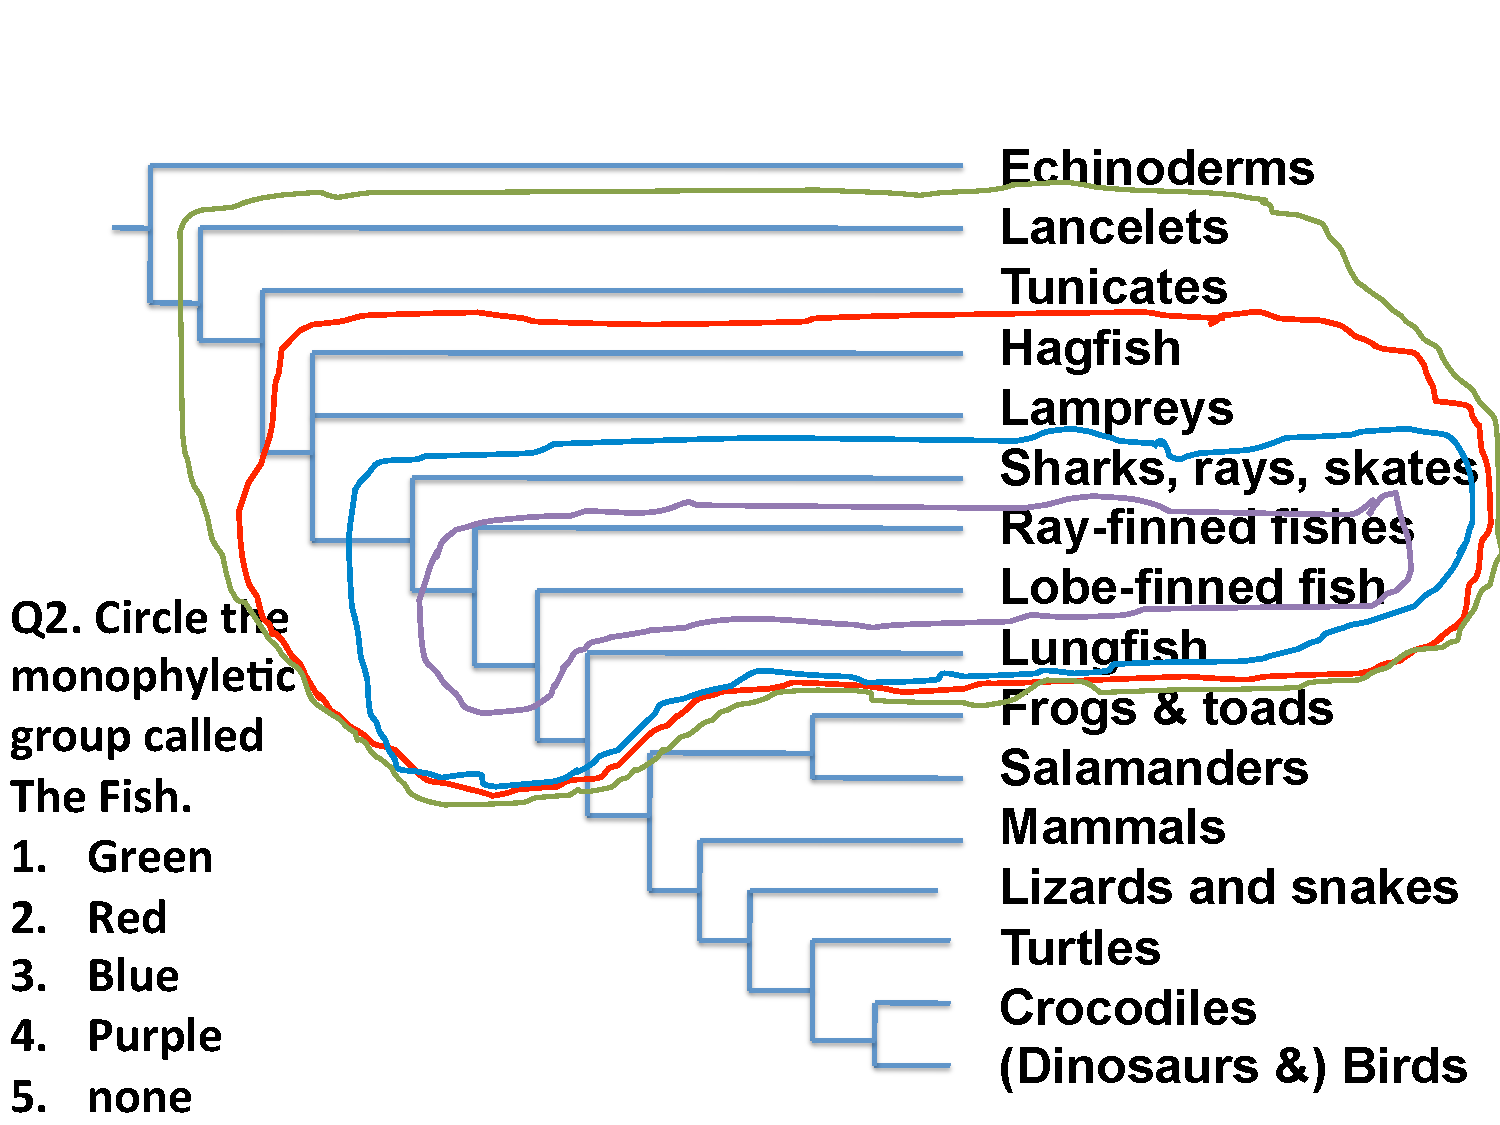
\includegraphics[width=\paperwidth]{./vertebrate-tree-clicker-slide.pdf}}
\begin{frame}[t,plain]
    \begin{adjustwidth}{-1.5em}{-1.5em}
        \cmask{Answer: 5}
    \end{adjustwidth}
\end{frame}
}
}

\begin{noheadline}
\begin{frame}
\frametitle{Today's issues:}
\vspace{5mm}
\tableofcontents[subsectionstyle=hide]
% \tableofcontents
\end{frame}
\end{noheadline}

\section{How do biologists recognize species?}

\begin{noheadline}
\begin{frame}[t]
    \frametitle{How do biologists recognize species?}
    \begin{adjustwidth}{-1.5em}{-1.5em}
        A species is a population, or group of populations, in which
        evolutionary forces are acting independently.

        \vspace{3mm}
        Speciation is a splitting event:

        \nbox{Note: because species can exist at large spatial scales, and the
            process of speciation occurs over long temporal scales, it is often
            difficult to delimit species in practice. I.e., species are easy to
            define, but hard to identify.}

        \vspace{4cm}
        \uncover<2->{
        Species are genetically isolated from each other.
        }
    \end{adjustwidth}
    \note[item]{Draw ``branch'' as ``population changing over time''; ask class
        to draw the splitting event.}
\end{frame}
\end{noheadline}

\begin{frame}[t]
    \begin{adjustwidth}{-1.5em}{-1.5em}
        Speciation occurs via:

        \begin{enumerate}
            \item Genetic isolation (lack of gene flow), followed by \ldots
            \item Genetic divergence (due to mutation, drift, and selection)
        \end{enumerate}

        \begin{itemize}
            \item Why does genetic isolation lead to ``evolutionary independent
                units?''
                
                \nbox{Once gene flow stops, the allele frequencies in each new
                    species are independent of one another. I.e., they are
                    ``free'' to evolve independently via mutation, drift, and
                    selection.}

                \vspace{5mm}
            \item Why does genetic divergence create synapomorphies?

                \nbox{Mutation will introduce new alleles (and traits) that are
                    unique to each new species (i.e., there is no gene flow to
                    ``share'' them). Thus, the descendants of each species will
                    accumulate unique alleles and traits.}

        \end{itemize}
    \end{adjustwidth}
\end{frame}

\subsection{Species criteria (``concepts'')}

\begin{frame}[t]
    \begin{adjustwidth}{-2em}{-1.5em}

    \vspace{-3mm}
    \textbf{Biological species concept:}
    \vspace{-3mm}
    \begin{table}%[htbp]
        \centering
        \begin{tabular}{ L{3.7cm} | L{3.7cm} | L{3.7cm} }
            Criterion for identifying species & Advantages & Disadvantages \\
            \hline
            \cmask{\mybullet Reproductive isolation (don't produce fertile offspring)} &
            \cmask{\mybullet Sound theoretically (lack of gene flow = evolutionarily
                independent)} &
            \cmask{\mybullet Doesn't apply to asexual species} \\
            \cmask{} &
            \cmask{} &
            \cmask{\mybullet Doesn't apply to fossils} \\
            \cmask{} &
            \cmask{} &
            \cmask{\mybullet Can be difficult to test} \\
            \cmask{} & \cmask{} & \cmask{} \\
            \cmask{} & \cmask{} & \cmask{} \\
            \cmask{} & \cmask{} & \cmask{} \\
            \cmask{} & \cmask{} & \cmask{} \\
            \cmask{} & \cmask{} & \cmask{} \\
            \cmask{} & \cmask{} & \cmask{} \\
            \cmask{} & \cmask{} & \cmask{} \\
            \cmask{} & \cmask{} & \cmask{} \\

        \end{tabular}
    \end{table}
    \end{adjustwidth}
\end{frame}

\begin{frame}[t]
    \begin{adjustwidth}{-2em}{-1.5em}

    \vspace{-3mm}
    \textbf{Morphospecies concept:}
    \vspace{-3mm}
    \begin{table}%[htbp]
        \centering
        \begin{tabular}{ L{3.7cm} | L{3.7cm} | L{3.7cm} }
            Criterion for identifying species & Advantages & Disadvantages \\
            \hline
            \cmask{\mybullet Distinct morphologically} &
            \cmask{\mybullet Widely applicable (sexual, asexual, fossils)} &
            \cmask{\mybullet Subjective (experts disagree what qualifies as
                ``distinct''} \\
            \cmask{} & \cmask{} & \cmask{} \\
            \cmask{} & \cmask{} & \cmask{} \\
        \end{tabular}
    \end{table}

    \vspace{2mm}
    \textbf{Phylogenetic species concept:}
    \vspace{-3mm}
    \begin{table}%[htbp]
        \centering
        \begin{tabular}{ L{3.7cm} | L{3.7cm} | L{3.7cm} }
            Criterion for identifying species & Advantages & Disadvantages \\
            \hline
            \cmask{\mybullet Smallest monophyletic groups} &
            \cmask{\mybullet Widely applicable (sexual, asexual, fossils)} &
            \cmask{\mybullet Difficult to apply; need to collect data and estimate trees} \\
            \cmask{} &
            \cmask{\mybullet Objective and testable} &
            \cmask{} \\
            \cmask{} & \cmask{} & \cmask{} \\
            \cmask{} & \cmask{} & \cmask{} \\
        \end{tabular}
    \end{table}
    \end{adjustwidth}
\end{frame}

\begin{frame}[t]
    \frametitle{An example of applying species concepts}
    \begin{adjustwidth}{-2em}{-1.5em}

        \begin{center} 
            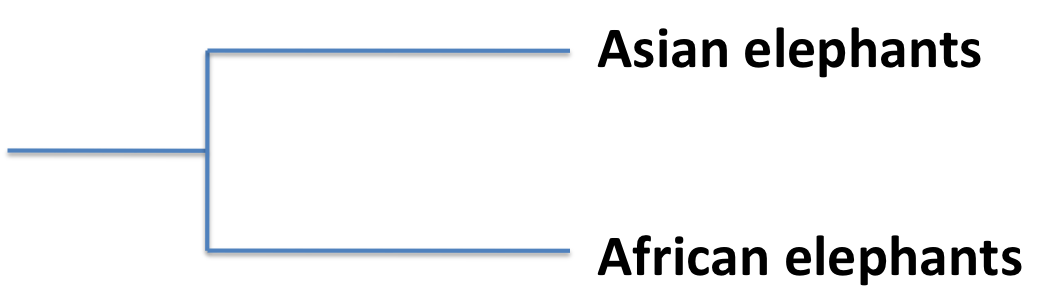
\includegraphics[width=0.8\linewidth]{elephant-tree-2-tips.png}
        \end{center}

        \begin{itemize}[<+->]
            \item Under morphospecies concept, African elephants were
                considered 1 species.
            \item Biological species concept is difficult to test with
                elephants!
        \end{itemize}
    \end{adjustwidth}
\end{frame}

\begin{frame}[t]
    \frametitle{An example of applying species concepts}
    \begin{adjustwidth}{-2em}{-1.5em}

        \begin{center} 
            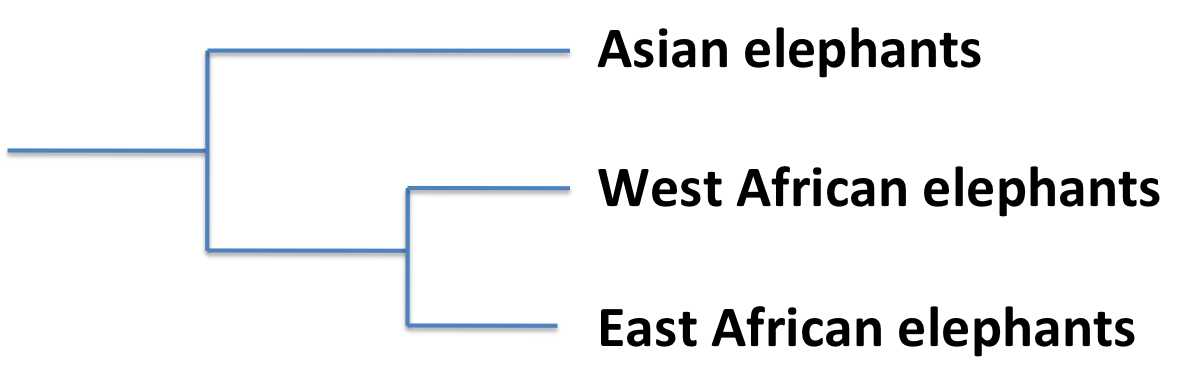
\includegraphics[width=0.8\linewidth]{elephant-tree-3-tips.png}
        \end{center}

        \begin{itemize}[<+->]
            \item DNA data revealed western and eastern populations had
                distinct alleles (synapomorphies) and were each monophyletic
                (statistical test rejected that they were not monophyletic).
            \item So, they are separate species according to the phylogenetic
                species concept!
            \item NOTE: If there was gene flow between the east and west
            populations, they would not be monophyletic (there would not be
            synapomorphies).
        \end{itemize}
    \end{adjustwidth}
\end{frame}

\clickerslide{
\begin{noheadline}
\begin{frame}
    \begin{adjustwidth}{-2em}{-1.5em}
    \begin{clickerquestion}
        \item The phylogeny below shows the relationships among populations of
            copepods called \textit{Eurytema affinis} (Go Dawgs!). How many
            phylogenetic species of \textit{E.\ affinis} are there? (Note that
            several populations exist at each tip.)
    \end{clickerquestion}

    \begin{columns}

        \column{0.1\linewidth}

        \begin{clickeroptions}
            \item 1
            \item 7
            \item \clickeranswer{8}
            \item 9
        \end{clickeroptions}

        \column{0.9\linewidth}

        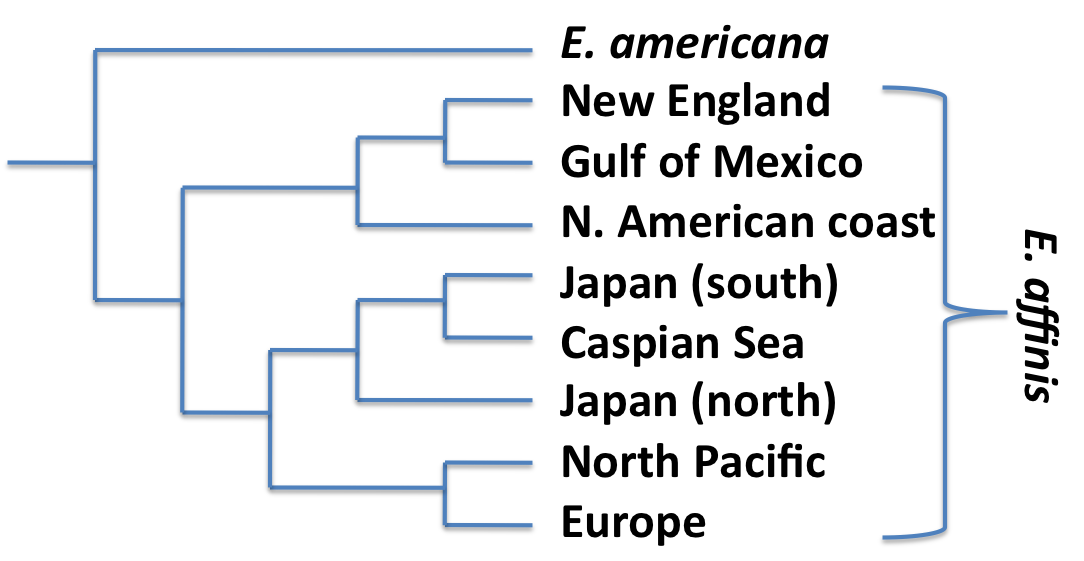
\includegraphics[width=1.0\columnwidth]{copepod-tree.png}

    \end{columns}
    \end{adjustwidth}
\end{frame}
\end{noheadline}
}

\section{How does speciation occur?}

\begin{noheadline}
\begin{frame}
\frametitle{Today's issues:}
\tableofcontents[currentsection,subsectionstyle=hide]
\end{frame}
\end{noheadline}

\subsection{Allopatric speciation}

\subsubsection{Dispersal}

\begin{frame}[t]
    \frametitle{Allopatric (``different land'') Speciation}
    \vspace{-4mm}
    \begin{adjustwidth}{-2em}{-1.5em}
        If populations are separated geographically, then evolutionary forces
        will act on them independently.
        \begin{uncoverenv}<2->
        \begin{enumerate}
            \item \textbf{Dispersal} (recall that genetic drift is very strong during
                founder events)
                \begin{itemize}
                    \item E.g., Iguanas of Anguilla
                        (\href{http://www.nature.com/news/1998/981015/full/news981015-3.html}{link})
                        \ldots Fiji, Galapagos, \ldots
                \end{itemize}
        \end{enumerate}
        \end{uncoverenv}
    \end{adjustwidth}

    \note[item]{1995, Hurricane Luis passed through Lesser Antilles. A floating
        mat of trees harbored 15 iguanas for more than 200 miles from
        Guadeloupe to Anguilla.}
\end{frame}

\begin{noheadline}
\begin{frame}[t]
    \begin{adjustwidth}{-2em}{-1.5em}
        \begin{columns}
            \column{0.3\linewidth}
            Hawaiian honeycreepers

            \column{0.7\linewidth}
            \begin{figure}
                \begin{center}
                    \includegraphics[width=\columnwidth]{../images/honeycreepers-labeled.jpg}
                    \caption{\tiny \copyright \href{http://www.hdouglaspratt.com/}{H.\ Douglas Pratt}}
                \end{center}
            \end{figure}
        \end{columns}
    \end{adjustwidth}
    \note[item]{Diverse monophyletic group of Hawaiian birds whose closest
        relatives are mainland finches}
\end{frame}
\end{noheadline}
\begin{noheadline}
\begin{frame}[t]
    \begin{adjustwidth}{-2em}{-1.5em}
    {\small Is this phylogeny of Hawaiian honeycreepers consistent with dispersal hypothesis?}
        \begin{figure}
            \begin{center}
                \includegraphics[width=\linewidth]{../images/honeycreeper-biogeography.jpg}
                \caption{\shortfullcite{Bromham2003}}
            \end{center}
        \end{figure}
    \end{adjustwidth}
    \note[item]{Yes! Outgroups (orange) are mainland finches. Phylogeny
        consistent with pattern of dispersal down island chain by age of island
        emergence!}
    \note[item]{Hawaiian silverswords and Drosophila show the same pattern}
\end{frame}
\end{noheadline}

\subsubsection{Vicariance}

\begin{frame}[t]
    \frametitle{Allopatric (``different land'') Speciation}
    \vspace{-4mm}
    \begin{adjustwidth}{-2em}{-1.5em}
        If populations are separated geographically, then evolutionary forces
        will act on them independently.
        \begin{enumerate}
            \item \textbf{Dispersal} (recall that genetic drift is very strong during
                founder events)
            \item \textbf{Vicariance:} Splitting an existing range into fragments
                \begin{itemize}
                    \item E.g., Death Valley pupfish
                \end{itemize}
        \end{enumerate}
    \end{adjustwidth}

    \note[item]{50,000 years ago Death Valley was rainy and had system of
        rivers and lakes. As lakes and rivers shrank, pupfish became isolated
        in tiny spring-fed oases. Each is now a distinct species.  Among rarest
        and most narrowly distributed species!}
\end{frame}


\subsection{Sympatric speciation}

\begin{frame}[t]
    \frametitle{Sympatric (``same land'') Speciation}
    \vspace{-4mm}
    \begin{adjustwidth}{-2em}{-1.5em}
        Can gene flow stop, or be reduced enough to initiate speciation, if
        populations are in the same geographic area?
        \begin{itemize}
            \item E.g., \textit{Mimulus lewisii} and \textit{M.\ cardinalis}
        \end{itemize}
        \begin{enumerate}
            \item \textbf{Mechanism of isolation:}

                \nbox{Disruptive selection for opposite ``extremes'' of
                    phenotype; hybrid individuals with intermediate trait
                    values have low fitness. E.g., in \textit{Mimulus},
                    selection for floral phenotypes that attract different
                    pollinators cuts off gene flow.}

                \vspace{5mm}
            \item \textbf{Mechanism of divergence:}

                \nbox{Once genetically isolated, evolutionary forces will be
                    independent in each new species, and differences
                    (synapomorphies) accumulate via mutation and continued
                    selection for alleles associated with divergent phenotypes
                    (drift too).}
        \end{enumerate}
    \end{adjustwidth}

\end{frame}

\begin{frame}[t]
    \frametitle{Sympatric (``same land'') Speciation}
    \vspace{-4mm}
    \begin{adjustwidth}{-2em}{-1.5em}
        \begin{itemize}
            \item E.g., \textit{Rhagoletis pomonella} (apple and hawthorn flies)
        \end{itemize}

        \begin{columns}

            \column{0.45\linewidth}

            \begin{enumerate}
                \item \textbf{Mechanism of isolation:}

                    \nbox{\small Disruptive selection for mating (and larval
                        feeding) on different fruit.}

                    \vspace{8mm}
                \item \textbf{Mechanism of divergence:}

                    \nbox{\small Once reproductively isolated due to different
                        mating sites, mutation and selection for feeding on
                        different fruits will cause differences
                        (synapomorphies) to accumulate (drift too).}
            \end{enumerate}

            \column{0.55\linewidth}
            
            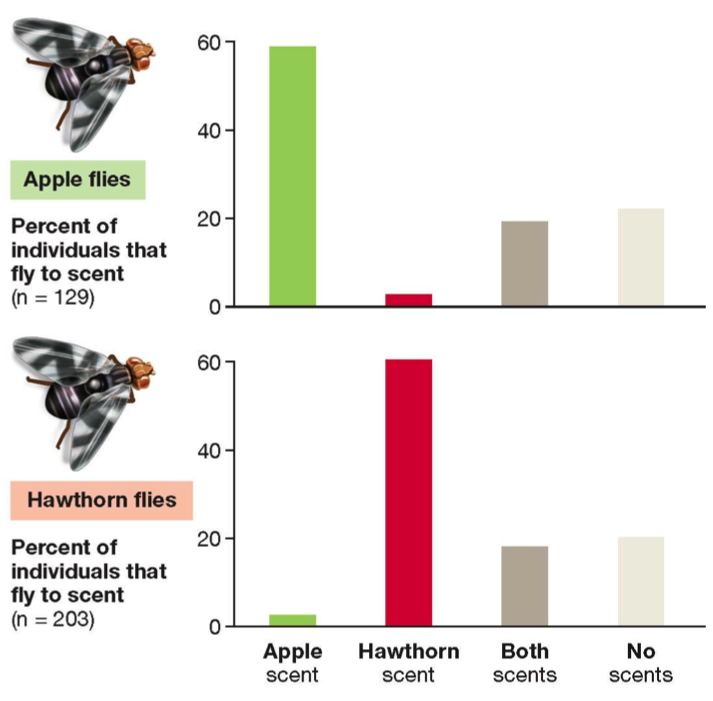
\includegraphics[width=\columnwidth]{rhagoletis.png}

        \end{columns}

    \end{adjustwidth}

\end{frame}

{
\usebackgroundtemplate{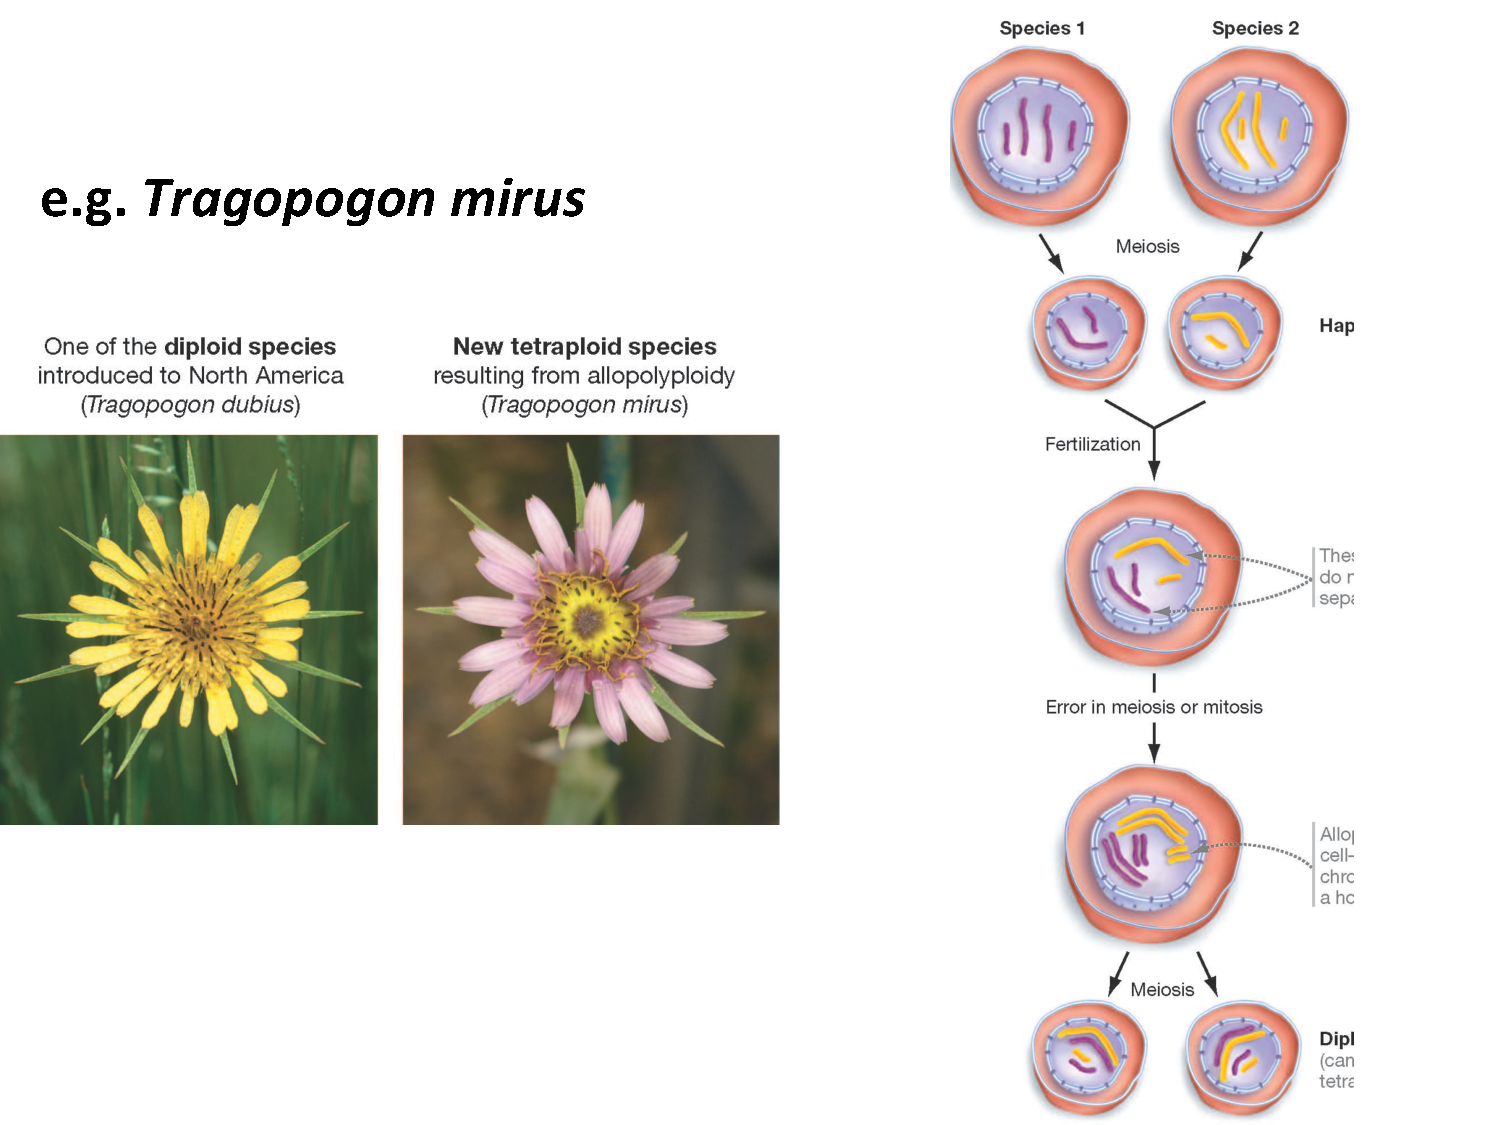
\includegraphics[width=\paperwidth]{./tragopogon-slide.pdf}}
\begin{frame}[plain]
    \note[item]{Found tetraploid species of goatsbeard in North America that is
        similar (intermediate) to two diploid species in the same area (both
        introduced from Europe)}
    \note[item]{Hypothesis: New species arose through hybridization.}
    \note[item]{Experiment: Cross diploid species in the lab.}
\end{frame}
}

\begin{frame}[t]
    \frametitle{Sympatric (``same land'') Speciation}
    \vspace{-4mm}
    \begin{adjustwidth}{-2em}{-1.5em}
        \begin{itemize}
            \item E.g., \textit{Tragopogon mirus}
        \end{itemize}
        \begin{enumerate}
            \item \textbf{Mechanism of isolation:}

                \nbox{\textbf{Polypoloidy} genetically isolated
                    \textit{Tragopogon mirus} from both diploid parental
                    species (crosses result in sterile triploids).}

                \vspace{9mm}
            \item \textbf{Mechanism of divergence:}

                \nbox{Mutation, selection, and drift will occur independently
                    in new species \ldots synapomorphies accumulate.}
        \end{enumerate}
    \vspace{12mm}
    Punchline: It is possible to study speciation (``macroevolution'')
    experimentally!
    \end{adjustwidth}

\end{frame}

\subsection[]{Mechanisms of isolation}

\subsection[]{Mechanisms of divergence}


\end{document}

\clickerslide{
\begin{frame}
    \begin{clickerquestion}
        \item 
        \begin{clickeroptions}
            \item 
            \item 
            \item 
            \item 
        \end{clickeroptions}
    \end{clickerquestion}
\end{frame}
}
